\section{Дифференцирование}
В прошлый раз определили $e^z$  доказали формулу $e^z = e^x(\cos y + i\,\sin y)$ для $z = x+ i\,y$. Показали, что $e^z$ имеет основной период $2\pi\,i$. Достаточно изучать экспоненту на основной полосе периода, то есть $\big\{z\colon y\in(-\pi,\pi)\big\}$. Легко видеть непрерывность. Возникает естественное обратное отображение $\ln (w) = \ln|w| + i\,\arg(w)$ (главная часть логарифма). Мы ввели обозначение $z\in\Ln w\iff w = e^z$. Увидели, что $\Ln w = \big\{\ln|w| + i\,(\arg w + 2\pi k)\big|k\in\Z\big\}$.

Доказали ещё теорему о производной обратной функции. Что даёт нам
\[
	(\ln w)'\big|_{w_0=e_{z_0}} = \frac1{(e^z)'\big|_{z=z_0}}=\frac1{e^{z_0}} = \frac1{w_0}.
\]
Пишем коротко $(\ln z)' = \frac1z$ для $z\in\C_-$.

Не все свойства логирифма переносятся из $\R$. Например, $\ln z^2\ne 2\ln z$, это странная функция.

Ещё одну функцию рассмотрим в качестве примера: $w = z^n$ для $n\ge 2$. Эта функция склеивает точки на одной окружности. Легко показать, что $(z^n)' = n z^{n-1}$. А что можно взять в качестве основной области? Нет простой периодичности, но есть инвариантность относительно поворотов.
\begin{figure}[H]
	\centering
	\begin{minitikZ}
		\axeS02\tikzPI{30}{-30}
		\draw (1,0) arc(0:30:1cm) node[anchor=west]{$\frac\pi n$};
		\draw[fill] (2,0)--(2.5,0) arc (0:10:2.5cm) -- (10:2) arc (10:0:2cm);
		\draw[dashed] (0,0)--(12:3.5);
		\draw[->] (3,0) arc (0:12:3cm) node[anchor=south]{$\gamma$};
	\end{minitikZ}
	$\mapS{z^n}$
	\begin{minitikZ}
		\axeS00
		\draw (-\hpW,0.1)--(0,0.1);
		\draw[dashed] (0,0)--(35:3.3);
		\draw[fill] (2,0)--(2.6,0) arc (0:25:2.6cm) -- (25:2) arc (25:0:2cm);
		\draw[->] (3,0) arc (0:35:3cm) node[anchor=west]{$n\gamma$};
	\end{minitikZ}
	\caption{Степенная функция}
	\label{fig9}
\end{figure}
Сегодня будем кратко обозначать $V:=V_{\left(-\frac\pi n,\frac\pi n\right)}$. $V$ при отображении $z^n$ перейдёт в $\C_-$. Рассмотрим $z(t) = t\cdot e^{i\gamma}$, $t>0$. Тогда $\big(z(t)\big)^n = t^n\cdot e^{i\,n\gamma}$. Есть обратная функция $z = \brancH{\sqrt[n]{w}} = \sqrt[n]{|w|}\cdot e^{\frac{i\,\arg w}n}$.
\begin{Task}
	$\Big(\brancH{\sqrt[n]z}\Big)'_{z_0} = \frac1{n z_0}\cdot \brancH{\sqrt[n]{z_0}}$, если короче, то $(\brancH{\sqrt[n]z})' = \frac1{nz}\brancH{\sqrt[n]z}$.
\end{Task}
\begin{Task}
	$\brancH{\sqrt[n]z} = e^{\frac1n\ln z}$.
\end{Task}
Просто по определению $\brancH{\sqrt[n]{z}} = \brancH{z^{\frac1n}}$.
\begin{Def}
	Пусть $\lambda\in\C$ "--- фиксированное число. Тогда $z^\lambda = e^{\lambda\Ln z}$ "--- многозначная функция. Можно доопределять в нуле по непрерывности.
\end{Def}
\begin{Task}
	Что будет, когда $\lambda\in\Z$? (Оказывается, будет однозначная функция.)
\end{Task}
\begin{Task}
	Что будет, когда $\lambda\in\Q$ (вещественные рациональные)?
\end{Task}
Для остальных $\lambda$ функция $z^n$ оказывается счётнозначной.
\begin{Task}
	Доказать, что $i^i\subset\R$.
\end{Task}
Что можем сказать про тригонометрические функции? $\cos z = \frac{e^{i\,z} + e^{-i\,z}}2$, $\sin z = \frac{e^{i\,z} - e^{-i\,z}}{2\,i}$ "--- $2\pi$-периодичные функции, а $\tg z = \frac{\sin z}{\cos z}$ и $\ctg z = \frac{\cos z}{\sin z}$ "--- $\pi$-периодичны. Но где они определены? Там, где знаменатели не обращаются в ноль.
\subsection{$\C$- и $\R$-линейные функции}
\begin{Def}
	Функция $w = l(z)$ называется $\C$-линейной, если
	\[
		\forall\ z_1,z_2,z,\lambda\in \C\pau l(z_1+z_2) = l(z_1) + l(z_2),\ l(\lambda z) = \lambda l(z).
	\]
\end{Def}
\begin{Task}
	$l(z)$ является $\C$-линейной, если и только если $\exists\ A\in\C\colon \forall\ z\in\C\pau l(z) = A\cdot z$.
\end{Task}
\begin{Def}
	Функция $w = L(z)$ называется $\R$-линейной, если
	\[
		\forall\ z_1,z_2,z\in\C,\ \forall\ \lambda\in\R\pau L(z_1+z_2) = L(z_1) + L(z_2),\ L(\lambda z) = \lambda L(z).
	\]
	Такие функции называются линйными формами.
\end{Def}
\begin{Task}
	$L(z)$ является $\R$-линейной, если и только если $\exists\ A,B\in\C\colon \forall\ z\in\C\pau L(z) = A\cdot z+B\cdot \ol z$.
\end{Task}
\begin{Task}
	Пусть есть $L(z) = A\,z+ B\,\ol z$ и $L_1(z) = A_1\,z+B_1\,\ol z$. Утверждается, что $L(z)\equiv L_1(z)\iff A = A_1$ и $B= B_1$.
\end{Task}
Надо просто решить систему. Очень просто получается.

\begin{Sl}
	$\R$-линейная функция $L(z) = A\,z + B\,\ol z$ является $\C$-линейной, если и только если $B=0$.
\end{Sl}
Давайте посмотрим, чему это соответствует, когда берём дифференциал от функции.

\begin{Def}
	Функция $w = f(z)$ (определённая в окрестности $U(z_0)$ точки $z_0\in\C$; в этой окрестности для любой точки $z$ определяем $\Delta z = z -z_0 = \Delta x + i\,\Delta y$) называется $\C$-дифференцируемой в точке $z_0$, если её полное приращение относительно $\Delta z$ представляется в виде
	\[
		\Delta f|_{z_0}(\Delta z)= f(z) - f(z_0) = A\cdot \Delta z + \ooo{\Delta z}{\Delta z\to0},
	\]
	где $A\in\C$ "--- постоянная. $A\cdot \Delta z$ называется главной линейной по $\Delta z$ частью приращения, обозначается $df|_{z_0}(\Delta z)\equiv A\cdot\Delta z$, и ещё называется дифференциалом $f$ в точке $z_0$. Таким образом, функция дифференцируема, если дифференциал является $\C$-линейной функцией относительно $\Delta z$.
\end{Def}

Рассмотрим предел $\yo{\Delta z}0\frac{\Delta f|_{z_0}(\Delta z)}{\Delta z}\overset{\exists}=f'(z_0)$. Очевидно выполнено
\begin{Sl}
	$f$ является $\C$-дифференцируемой, если и только если существует $f'|_{z_0}$ и тогда $A = f'_{z_0}$.
\end{Sl}

Рассмотрим функцию $f(z) = z\ol z = |z|^2 = x^2 + y^2$. Уж куда проще. Фиксируем точку $z_0\ne0$.
\[
	\Delta f|_{z_0}(\Delta z) = (z_0+\Delta z)(\ol z_0+\ol{\Delta z}) - z_0\ol z_0 = 
	\underbrace{\ol z_0}_{A}\Delta z_0 + 
	\underbrace{z_0}_B\ol{\Delta z} + 
	\underbrace{|\Delta z|^2}{\oo(|\Delta z|)}.
\]
При этом $\oo(\Delta z) = \oo\big(|\Delta z|\big) = \oo\big(\sqrt{\Delta x^2+\Delta y^2}\big)$. Так как $B\ne0$, $f$ не является $\C$-дифференцируемой функцией в точке $z_0$.

Пусть $f$ определена в окрестности $U(z_0)$ точки $z_0\in\C$. $z = x+i\,y$, $\Delta z = z - z_0 = \Delta x + i\,\Delta y$.
\begin{figure}[H]
	\centering
	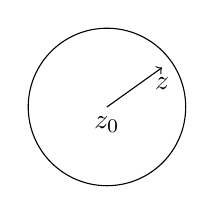
\begin{tikzpicture}
		\draw(0,0) circle (1cm);
		\draw(0,0) node[anchor=north]{$z_0$};
		\draw[->] (0,0)--(0.7,0.5) node[anchor=north]{$z$};
	\end{tikzpicture}
	\caption{Окрестность "--- выпуклое множество}
	\label{fig9}
\end{figure}
Можно на какое-то время забывать про $i$ и считать, что $f(x)$ "--- это функция на плоскости $f(x,y)=u(x,y) + i\, v(x,y)$, $u = \Re f$, $v= \Im f$.

Например, для $f(z) = e^z$ имеем $u(x,y) = e^x\cos y$, $v(x,y) = e^x\sin y$. Для $f(z) = z^2$ имеем $u(x,y) = x^2 - y^2$, $v(x,y) = 2xy$.

Пусть $u,v$ для некоторой $f(z)$ определены в окрестности точки $(x_0,y_0)\sim z_0$.
\begin{Def}
	Функция $f$ называется $\R$-дифференцируемой в точке $z_0$, если функции $u(x,y)$ и $v(x,y)$ одновременно являются дифференцируемыми функциями $2$-х вещественных переменных $( x,y)$ в точке $z_0 = (x_0,y_0)$, то есть
	\[
		\Delta u|_{z_0}(\Delta z) = u(x_0+\Delta x,y_0+\Delta y) - u(x_0,y_0) = 
		\underbrace{\CP ux\bigg|_{z_0}}_{u'_x|_{z_0}}\cdot\Delta x + 
		\underbrace{\CP uy\bigg|_{z_0}}_{u'_y|_{z_0}}\cdot\Delta y +
		\underbrace{\oo(\Delta z)}_{\oo\left(\sqrt{x^2+y^2}\right)}
	\]
	и одновременно
	\[
		\Delta v|_{z_0}(\Delta z) = v(x_0+\Delta x,y_0+\Delta y) - v(x_0,y_0) = 
		\underbrace{\CP vx\bigg|_{z_0}}_{v'_x|_{z_0}}\cdot\Delta x + 
		\underbrace{\CP vy\bigg|_{z_0}}_{v'_y|_{z_0}}\cdot\Delta y +
		\underbrace{\oo(\Delta z)}_{\oo\left(\sqrt{x^2+y^2}\right)}.
	\]
\end{Def}
Бывают функции, не являющиеся $\R$-дифференцируемыми. Для этого достаточно, чтобы хотя бы $u$ не была дифференцируемой в $\R^2$.
\begin{figure}[H]
	\centering
	\begin{tikzpicture}
		\axeS00
		\draw	(0,0) node[anchor=north east]{$0$};
		\draw	(3,0) node[anchor=south]{$0$};
		\draw	(0,-2) node[anchor=east]{$0$};
		\draw	(0,1.5) node[anchor=east]{$0$};
		\draw	(-2,1) node{$1$};
		\draw	(2,1) node{$1$};
		\draw	(-2,-1) node{$1$};
		\draw	(2,-1) node{$1$};
	\end{tikzpicture}
	\caption{Функция не диффенцируемы в $\R^2$}
	\label{fig10}
\end{figure}
Частная производная работает только по двум направлениям, а дифференциал работает по всем.

Приращение можно записать ещё в таком виде.
\[
	\Delta f|_{z_0}(\Delta z) = \Delta u|_{z_0}+i\,\Delta v|_{z_0}(\Delta z) =
	\underbrace{(u'_x+i\,v'_x)|_{z_0}}_{f'_x|_{z_0}}\cdot \Delta x +
	\underbrace{(u'_y+i\,v'_y)|_{z_0}}_{f'_y|_{z_0}}\cdot \Delta y +
	\ooo{\Delta z}{\Delta z\to0}.
\]
Возникают ествественные частные производные. А теперь идея такая. Давайте в этом выражении заменим $(x,y)\to(z,\ol z)$.
\[
	\Delta z = \Delta x + i\,\Delta y;\quad 
	\ol{\Delta z} = \Delta x - i\,\Delta y;\quad 
	\Delta x = \frac{\Delta z + \ol{\Delta z}}2;\quad
	\Delta y = \frac{\Delta z - \ol{\Delta z}}{2\,i}.
\]
После подстановки возникают естественные определения для $\CP fz$ и $\CP f{\ol z}$.
\begin{multline*}
	\Delta f|_{z_0}(\Delta z) = 
	 f'_x|_{z_0}\left(\frac{\Delta z+ \ol{\Delta z}}{2}\right) + 
	 f'_y|_{z_0}\left(\frac{\Delta z- \ol{\Delta z}}{2\,i}\right) + 
	 \ooo{\Delta z}{\Delta z\to 0} =\\=
	\frac12\underbrace{(f'_x-i\,f'_y)|_{z_0}}_{\left.\CP fz\right|_{z_0}}\cdot\Delta z+
	\frac12\underbrace{(f'_x+i\,f'_y)|_{z_0}}_{\left.\CP f{\ol z}\right|_{z_0}}\cdot\ol{\Delta z} + 
	 \ooo{\Delta z}{\Delta z\to 0} =
	 \CP fz\bigg|_{z_0}\Delta z + \CP f{\ol z}\ol{\Delta z}+
	 \ooo{\Delta z}{\Delta z\to 0}.
 \end{multline*}
\begin{Def}
В случае $\R$-дифференцируемости, главная линейная часть приращения имеем вид
\[
	 \CP fz\bigg|_{z_0}\Delta z + \CP f{\ol z}\ol{\Delta z},
 \]
 то есть является $\R$-линейной функцией по $\Delta z$. Её обозначают $df|_{z_0}(\Delta z)$.
\end{Def}
\begin{Sl}
	$\R$-дифференцируемая функция $f$ в точке $z_0$ является $\C$-дифференцируемой в точке $z_0$, если и только если $\CP f{\ol z}\Big|_{z_0}=0$, если и только если $\exists\ f'(z_0)$.
\end{Sl}
Напишем критерий $\C$-дифференцируемости в более понятных терминах.
\[
	2\CP f{\ol z}\bigg|_{z_0} = \big(u'_x + i\,v'_x + i(u'_y + i\,v'_y)\big)\big|_{z_0} = 0\iff
	\begin{cases}
		u'_x - v'_y = 0;\\ v'_x+ u'_y = 0.
	\end{cases}
\]
У этого критерия есть название.
\begin{The}[Коши"--~Римана]
	Пусть $f = u+i\,v$ является $\R$-дифференцируемой в точке $z_0$. Тогда $f$ $\C$-дифференцируема в $z_0$, если и только если $\exists\ f'(z_0)\iff$
	\[
		\begin{cases}
			u'_x = v'_y;\\ u'_y=-v'_x.
		\end{cases}
	\]
\end{The}
Бывает так, что только одна точка хорошая. Например, $f(z) = x^2 +y^2 = z\ol z$. Только в нуле есть комлексная производная.
\begin{Zam}
	Пусть $f$ является $\R$-дифференцируемой в точке $z_0$. Пусть $\Delta z = \Delta x + i\,\Delta y = \underbrace{|\Delta z|}_{\ne0} e^{i\,\theta}$, где $\theta = \arg(\Delta z)$ "--- фиксирована. Рассмотрим предел
	\[
		\lim\limits_{\substack{\Delta z\to0 \\ \arg(\Delta z)=\theta}}\frac{\Delta f|_{z_0}(\Delta z)}{\Delta z}.
	\]
Он является производной $f$  по направлению $e^{i\,theta}$, где $\theta\in(-\pi,\pi]$. Что получим, если этот пределе преобразуем, используя $\R$-дифференцируемость:
\[
		\lim\limits_{\substack{\Delta z\to0 \\ \arg(\Delta z)=\theta}}\frac{\Delta f|_{z_0}(\Delta z)}{\Delta z}=
		\lim\limits_{\substack{\Delta z\to0 \\ \arg(\Delta z)=\theta}}
			\frac{\left.\CP fz\right|_{z_0}\Delta z + \left.\CP f{\ol z}\right|_{z_0}\ol{\Delta z} + \oo(\Delta z)}{|\Delta z|e^{i\,\theta}}=
			\CP fz\bigg|_{z_0} + \CP f{\ol z}\bigg|_{z_0}e^{-2\,i\,\theta},
		\]
		так как $\ol{\Delta z} = \Delta x - i\,\Delta y = |\Delta z|e^{-i\,\theta}$.
\end{Zam}
Получается следующее замечательное следствие.
\begin{Sl}
В указанных обозначениях совокупность всех производных по направлению дважды пробегает (по часовой стрелке) окружность с центром $\CP fz\Big|_{z_0}$ и радиусом $\bigg|\CP f{\ol z}\Big|_{z_0}\bigg|$ при $\theta$, один раз пробегающей $(-\pi,\pi]$.
\end{Sl}
\begin{Sl}
	Все производные по направлению $\CP f{z_\theta}\Big|_{z_0}$ совпадают, если и только если $\CP f{\ol z}\Big|_{z_0}=0$. В этом случае все они равны $\CP fz\Big|_{z_0}$ и совпадают с $f'(z_0) = :\DP fz\Big|_{z_0}$.
\end{Sl}
